\documentclass[11pt]{article}
\usepackage[a4paper,margin=2cm]{geometry}
\usepackage[T1]{fontenc}
\usepackage{helvet}
\renewcommand{\familydefault}{\sfdefault}
\usepackage{xcolor}
\usepackage{tikz}
\usetikzlibrary{arrows.meta,positioning,shapes.callouts,decorations.pathmorphing,calc}
\usepackage{graphicx}
\usepackage{booktabs}
\usepackage{tabularx}
\usepackage{array}
\usepackage{enumitem}
\usepackage{parskip}
\usepackage[hidelinks]{hyperref}
\setlist{nosep,leftmargin=1.4em}
\renewcommand{\arraystretch}{1.25}

\definecolor{cE}{HTML}{2F7FD6}   % eMBB
\definecolor{cU}{HTML}{6A1FB5}   % URLLC
\definecolor{cM}{HTML}{E8792C}   % mMTC
\definecolor{ok}{HTML}{2C6E49}
\definecolor{bad}{HTML}{B3261E}
\definecolor{soft}{HTML}{EEF3F6}
\definecolor{ink}{HTML}{1F2D3D}
\definecolor{grey}{HTML}{5A6570}

\graphicspath{{../screenshots/open5gs/}}

% ───────────── stick figures ─────────────
% \person[<tikz options>]{<x,y>}{<arms: down|up|point|wave|hold|shrug>}
\tikzset{stick/.style={line width=1.3pt,line cap=round,line join=round}}
\newcommand{\person}[3][]{%
  \begin{scope}[shift={(#2)},stick,#1]
    \draw (0,1.55) circle (0.22);
    \draw (-0.07,1.6) circle (0.012) (0.07,1.6) circle (0.012);
    \draw (-0.09,1.49) .. controls (-0.03,1.43) and (0.03,1.43) .. (0.09,1.49);
    \draw (0,1.33) -- (0,0.6);
    \draw (0,0.6) -- (-0.25,0) (0,0.6) -- (0.25,0);
    \ifx#3u\draw (0,1.15) -- (-0.35,1.55) (0,1.15) -- (0.35,1.55);\fi
    \ifx#3d\draw (0,1.15) -- (-0.3,0.75) (0,1.15) -- (0.3,0.75);\fi
    \ifx#3p\draw (0,1.15) -- (-0.3,0.75) (0,1.15) -- (0.5,1.2);\fi
    \ifx#3w\draw (0,1.15) -- (-0.3,0.75) (0,1.15) -- (0.3,1.5);\fi
    \ifx#3h\draw (0,1.15) -- (0.35,0.95) -- (0.45,1.05) (0,1.15) -- (-0.3,0.75);\fi
    \ifx#3s\draw (0,1.15) -- (-0.3,1.1) -- (-0.4,1.3) (0,1.15) -- (0.3,1.1) -- (0.4,1.3);\fi
  \end{scope}}
\newcommand{\say}[3][]{\node[draw,rounded corners=4pt,fill=white,font=\footnotesize,align=center,inner sep=3pt,#1] at (#2) {#3};}
\newcommand{\server}[3]{% <x,y> <colour> <label>
  \begin{scope}[shift={(#1)}]
    \draw[#2,fill=#2!12,line width=1pt,rounded corners=2pt] (-0.45,0) rectangle (0.45,0.9);
    \foreach \yy in {0.2,0.45,0.7} \draw[#2] (-0.3,\yy) -- (0.3,\yy);
    \node[font=\scriptsize\bfseries,#2] at (0,-0.22) {#3};
  \end{scope}}

\newcommand{\shot}[3]{\par\noindent\begin{minipage}{\linewidth}\centering\includegraphics[width=#1\linewidth]{#2}\par\vspace{3pt}{\footnotesize #3}\end{minipage}\par\medskip}
\newcommand{\proof}[1]{\par{\footnotesize\color{grey}Proof: \texttt{#1}}\par}
\newenvironment{keybox}{\par\noindent
\begin{tikzpicture}\node[fill=soft,rounded corners=6pt,inner sep=8pt,text width=0.95\linewidth]\bgroup}{\egroup;\end{tikzpicture}\par}

\begin{document}

% ═════════════════════════ cover ═════════════════════════
\begin{center}
{\LARGE\bfseries\color{ink} The two orchestrators, explained with stick figures}\\[4pt]
{\large Phase 2b — what we built, what we measured, and where the proof is}\\[2pt]
{\color{grey}Team 23UG005 · Open5GS stack, 100 UEs · 8 October 2026}
\end{center}

\begin{center}
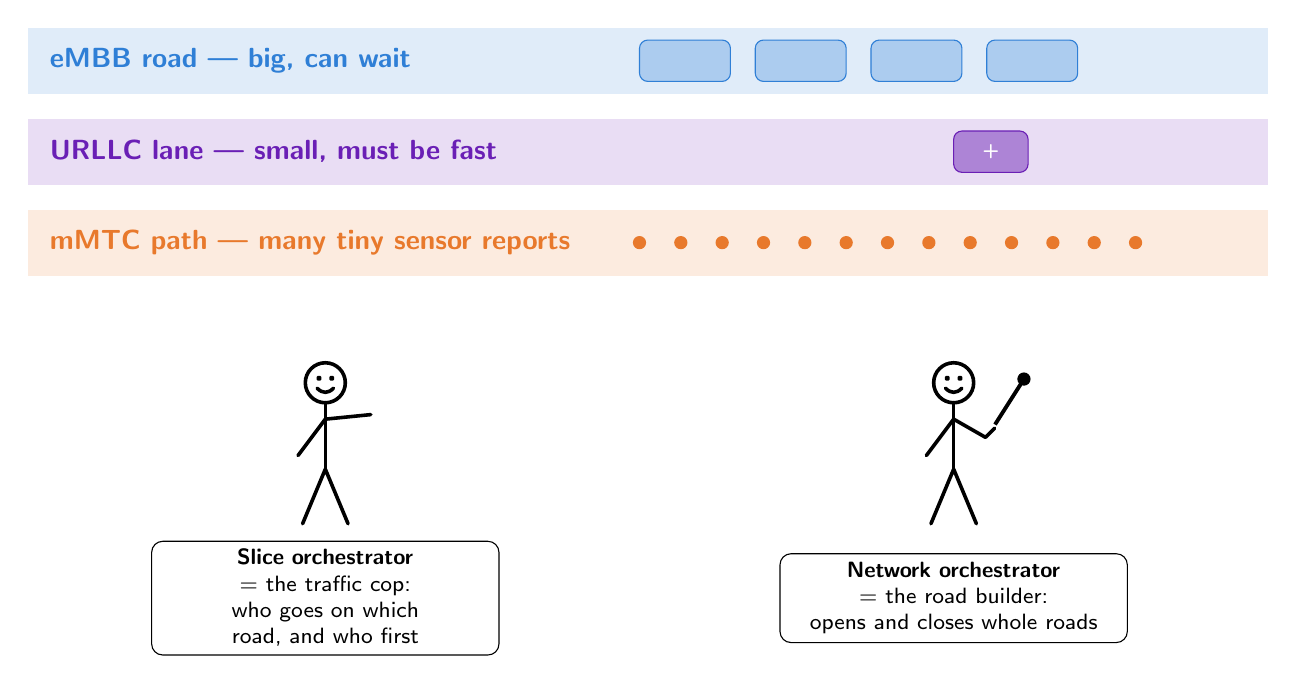
\begin{tikzpicture}[scale=1.05]
  % three roads
  \fill[cE!15] (0,3.0) rectangle (15,3.8); \node[cE,font=\bfseries,anchor=west] at (0.15,3.4) {eMBB road — big, can wait};
  \fill[cU!15] (0,1.9) rectangle (15,2.7); \node[cU,font=\bfseries,anchor=west] at (0.15,2.3) {URLLC lane — small, must be fast};
  \fill[cM!15] (0,0.8) rectangle (15,1.6); \node[cM,font=\bfseries,anchor=west] at (0.15,1.2) {mMTC path — many tiny sensor reports};
  \foreach \x in {7.4,8.8,10.2,11.6} \draw[cE,fill=cE!40,rounded corners=3pt] (\x,3.15) rectangle ++(1.1,0.5);
  \draw[cU,fill=cU!55,rounded corners=3pt] (11.2,2.05) rectangle ++(0.9,0.5);
  \node[white,font=\scriptsize\bfseries] at (11.65,2.3) {+};
  \foreach \x in {7.4,7.9,...,13.4} \fill[cM] (\x,1.2) circle (0.08);
  % traffic cop
  \person[scale=1.1]{3.6,-2.2}{p}
  \say[text width=4.2cm]{3.6,-3.1}{\textbf{Slice orchestrator}\\= the traffic cop:\\who goes on which road, and who first}
  % builder
  \person[scale=1.1]{11.2,-2.2}{h}
  \draw[line width=1.4pt] (11.7,-1.0) -- (12.05,-0.45); \fill (12.05,-0.45) circle (0.08);
  \say[text width=4.2cm]{11.2,-3.1}{\textbf{Network orchestrator}\\= the road builder:\\opens and closes whole roads}
\end{tikzpicture}
\end{center}

\begin{keybox}
\textbf{In one paragraph.} Our 5G network has three slices, like three roads. The \textbf{slice
orchestrator} is the traffic cop: it decides which road each request uses, lets VIPs (critical
devices) go first, and slows down the big road when it starts hurting the fast lane. The
\textbf{network orchestrator} is the road builder: it opens a whole road when someone needs it,
closes it when nobody does, checks every step, and undoes its work if something goes wrong.
Everything below was measured on our running 100-UE stack, and every number has a file behind it.
\end{keybox}

\vspace{4pt}
\textbf{Contents}\quad
1~The setup \quad 2~Traffic cop: priority \quad 3~Traffic cop: the feedback controller \quad
4~Traffic cop: planning \quad 5~Road builder: off and on \quad 6~Road builder: rollback \quad
7~Road builder: on its own (closed loop) \quad 8~Road builder: compute \quad
9~The photos: one live run \quad 10~Things that went wrong \quad 11~Where every proof lives

\newpage
% ═════════════════════════ 1 setup ═════════════════════════
\section{The setup: 100 phones and sensors, three slices}

\begin{center}
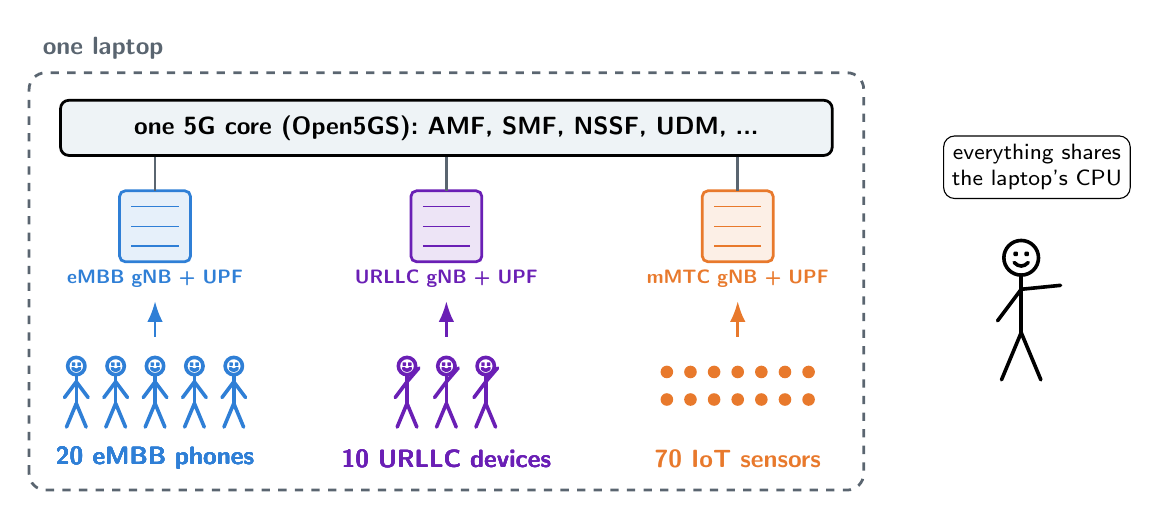
\begin{tikzpicture}
  \foreach \i in {0,...,4} \person[cE,scale=0.5]{0.2+\i*0.5,0}{d}
  \node[cE,font=\small\bfseries] at (1.2,-0.4) {20 eMBB phones};
  \foreach \i in {0,...,2} \person[cU,scale=0.5]{4.4+\i*0.5,0}{w}
  \node[cU,font=\small\bfseries] at (4.9,-0.4) {10 URLLC devices};
  \foreach \i in {0,...,6} \fill[cM] (7.7+\i*0.3,0.35) circle (0.08);
  \foreach \i in {0,...,6} \fill[cM] (7.7+\i*0.3,0.7) circle (0.08);
  \node[cM,font=\small\bfseries] at (8.6,-0.4) {70 IoT sensors};
  \foreach \x/\c in {1.2/cE,4.9/cU,8.6/cM} \draw[-{Latex},line width=1pt,\c] (\x,1.15) -- (\x,1.6);
  \server{1.2,2.1}{cE}{eMBB gNB + UPF}
  \server{4.9,2.1}{cU}{URLLC gNB + UPF}
  \server{8.6,2.1}{cM}{mMTC gNB + UPF}
  \foreach \x in {1.2,4.9,8.6} \draw[line width=1pt,grey] (\x,3.0) -- (\x,3.45);
  \draw[line width=1pt,fill=soft,rounded corners=3pt] (0,3.45) rectangle (9.8,4.15);
  \node[font=\small\bfseries] at (4.9,3.8) {one 5G core (Open5GS): AMF, SMF, NSSF, UDM, ...};
  \draw[line width=1pt,dashed,grey,rounded corners=6pt] (-0.4,-0.8) rectangle (10.2,4.5);
  \node[grey,font=\small\bfseries,anchor=south west] at (-0.35,4.55) {one laptop};
  \person{12.2,0.6}{p}
  \say{12.4,3.3}{everything shares\\the laptop's CPU}
\end{tikzpicture}
\end{center}

Each slice has its own radio (gNB), its own user-plane (UPF) and its own data network. What they
\emph{share} is the laptop's CPU. Remember that — it turns out to matter in section 3.

% ═════════════════════════ 2 priority ═════════════════════════
\section{Traffic cop: priority inside URLLC (ARP)}

\begin{center}
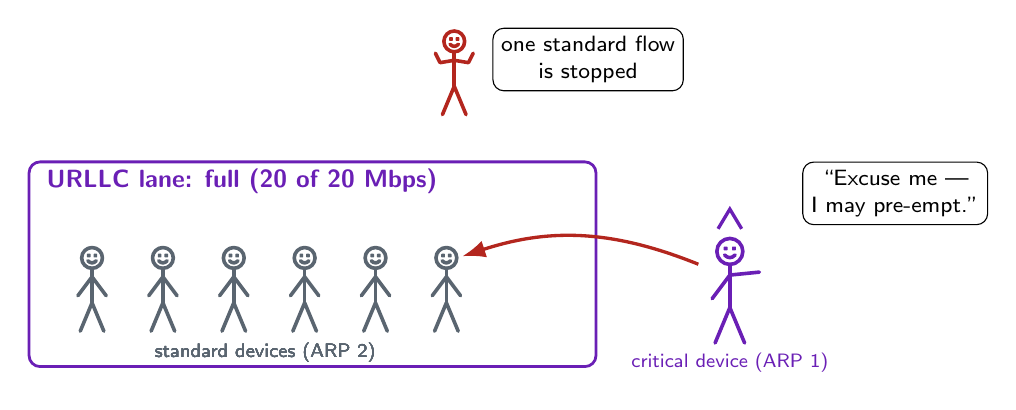
\begin{tikzpicture}
  \draw[cU,line width=1pt,rounded corners=4pt] (-0.4,-0.3) rectangle (6.8,2.3);
  \node[cU,font=\small\bfseries,anchor=west] at (-0.3,2.05) {URLLC lane: full (20 of 20 Mbps)};
  \foreach \i in {0,...,5} \person[scale=0.6,grey]{\i*0.9+0.4,0.15}{d}
  \node[font=\scriptsize,grey] at (2.6,-0.12) {standard devices (ARP 2)};
  \person[cU,scale=0.75]{8.5,0}{p}
  \draw[cU,line width=1.2pt] (8.35,1.45) -- (8.5,1.7) -- (8.65,1.45);  % crown
  \node[font=\scriptsize,cU] at (8.5,-0.25) {critical device (ARP 1)};
  \draw[-{Latex},line width=1.2pt,bad] (8.1,1.0) to[bend right=20] (5.1,1.1);
  \say{10.6,1.9}{``Excuse me —\\I may pre-empt.''}
  \person[scale=0.6,bad]{5.0,2.9}{s}
  \say{6.7,3.6}{one standard flow\\is stopped}
\end{tikzpicture}
\end{center}

3GPP has a rule for exactly this: \textbf{ARP} (Allocation and Retention Priority). We gave 3 of
the 10 URLLC devices ARP 1 (``critical, may pre-empt'') and 7 of them ARP 2 (``standard, may be
pre-empted''). The rule is stored in each device's subscription in the core.

\begin{tabularx}{\linewidth}{@{}lX@{}}
\toprule
\textbf{What we did} & \textbf{What happened} \\ \midrule
20 standard demands & all admitted — the lane is full (20/20 Mbps) \\
1 more standard demand & \textbf{refused}: an equal priority cannot push anyone out \\
5 critical demands & \textbf{all admitted}, each by stopping exactly \textbf{one} standard flow \\
the flows afterwards & critical 5/5 got their full rate; the 15 standard flows left also got theirs \\
\bottomrule
\end{tabularx}
We ran it twice and got the same result both times.
\proof{docs/evidence/open5gs-orchestrator-dynamic/1-priority.txt}

\shot{0.82}{13-demands-by-arp-priority.png}{Grafana, from the live run in section 9: demands per minute by ARP level. ``URLLC ARP 1 admitted'' is the critical devices; ``URLLC ARP 2 preempted'' is the standard flows they pushed out.}

% ═════════════════════════ 3 controller ═════════════════════════
\newpage
\section{Traffic cop: the feedback controller}

\begin{center}
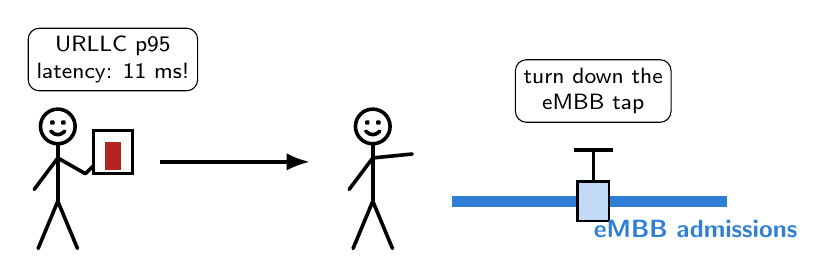
\begin{tikzpicture}
  \person{0,0}{h}
  \draw[line width=1pt,fill=white] (0.45,0.95) rectangle (0.95,1.5);
  \fill[bad] (0.6,1.0) rectangle (0.8,1.35);
  \say{0.7,2.4}{URLLC p95\\latency: 11 ms!}
  \draw[-{Latex},line width=1.2pt] (1.3,1.1) -- (3.2,1.1);
  \person{4,0}{p}
  \draw[cE,line width=4pt] (5,0.6) -- (8.5,0.6);
  \draw[line width=1pt,fill=cE!30] (6.6,0.35) rectangle (7.0,0.85);
  \draw[line width=1.2pt] (6.8,0.85) -- (6.8,1.25) (6.55,1.25) -- (7.05,1.25);
  \say{6.8,2.0}{turn down the\\eMBB tap}
  \node[cE,font=\small\bfseries] at (8.1,0.25) {eMBB admissions};
\end{tikzpicture}
\end{center}

Every 5 seconds the controller looks at URLLC's latency (the 95th percentile over the last 10 s).
If it goes above 8 ms (80\,\% of the 10 ms budget), it \textbf{cuts} how much eMBB traffic is
admitted. When things are calm again and eMBB wants more, it \textbf{raises} the limit a little.
That is the same ``cut fast, grow slowly'' rule TCP uses (AIMD).

\textbf{Why eMBB? We measured it.} Each kind of traffic alone, controller off:

\begin{tabularx}{\linewidth}{@{}Xccc@{}}
\toprule
\textbf{Load (120 s)} & \textbf{URLLC p95} & \textbf{URLLC p99} & \textbf{host load} \\ \midrule
nothing (idle) & 2.5 ms & 5.4 ms & 2.3 \\
URLLC demand only & 2.8 ms & 5.3 ms & 5.0 \\
eMBB demand only & \textbf{8.9 ms} & \textbf{17.5 ms} & 36.9 \\
\bottomrule
\end{tabularx}
\proof{docs/evidence/open5gs-orchestrator-dynamic/4-diagnosis.txt}

URLLC's own traffic does not slow URLLC down. eMBB's does — through the CPU they share.

\textbf{The result — same demand, controller off vs on (180 s each):}

\begin{tabularx}{\linewidth}{@{}Xcc@{}}
\toprule
& \textbf{controller off} & \textbf{controller on} \\ \midrule
eMBB flows that got their full rate & 68\,\% & \textbf{\color{ok}100\,\%} \\
URLLC latency mean / p95 / p99 & 5.1 / 20.5 / 55.4 ms & \textbf{\color{ok}3.2 / 12.5 / 34.0 ms} \\
URLLC flows that got their full rate & 100\,\% & 100\,\% \\
eMBB data actually delivered & 266 Mbps & 109 Mbps \\
\bottomrule
\end{tabularx}
\proof{docs/evidence/open5gs-orchestrator-dynamic/2-comparison.txt}

\begin{keybox}
\textbf{Honest note.} The controller makes every admitted eMBB flow work and cuts URLLC's slow tail
by about 40\,\%, but it does \emph{not} keep URLLC under the 10 ms target the whole time on this
laptop, and it costs eMBB volume. Much of that ``266 Mbps'' was broken flows, though.
\end{keybox}

\shot{0.82}{12-controller-watches-urllc-p95.png}{What the controller watches (live run, section 9): URLLC p95 over the last 10 s. Each time it climbs over the yellow 8 ms line, the controller cuts eMBB, and it comes back down.}
\shot{0.82}{10-embb-capacity-limit-admitted-measured.png}{eMBB in the same run: the policy capacity (green, 500 Mbps) and the controller's admission limit (yellow) falling from 500 to 50–130 Mbps under load. The jump back to 500 at 16:11:20 is the orchestrator being restarted for the priority test, not the controller.}

% ═════════════════════════ 4 planning ═════════════════════════
\medskip
\section{Traffic cop: planning — how many roads do we need?}

\begin{center}
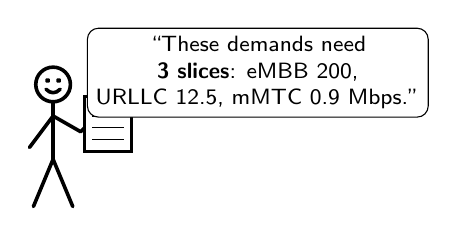
\begin{tikzpicture}
  \person{0,0}{h}
  \draw[line width=1pt,fill=white] (0.4,0.7) rectangle (1.0,1.4);
  \foreach \yy in {0.85,1.0,1.15,1.3} \draw (0.5,\yy) -- (0.9,\yy);
  \say{2.6,1.7}{``These demands need\\\textbf{3 slices}: eMBB 200,\\URLLC 12.5, mMTC 0.9 Mbps.''}
\end{tikzpicture}
\end{center}

\texttt{/plan} looks at a set of demands (or what it actually saw in the last few minutes) and says
which slices are needed and how much capacity each needs. Every kind of traffic goes on the
cheapest road that is still good enough.

\begin{tabularx}{\linewidth}{@{}Xcl@{}}
\toprule
\textbf{Demand} & \textbf{slices needed} & \textbf{capacity needed} \\ \midrule
Phase 2b mix: 10 control, 20 video, 70 sensors & 3 & eMBB 200, URLLC 12.5, mMTC 0.88 Mbps \\
only video and files (can wait) & \textbf{1} & eMBB 487.5 Mbps \\
what the orchestrator saw in a 180 s run & 2 & eMBB 363, URLLC 13.5 Mbps \\
\bottomrule
\end{tabularx}
\proof{docs/evidence/open5gs-orchestrator-dynamic/3-planning.txt}

The road builder (next sections) is the one who \emph{acts} on this answer.

% ═════════════════════════ 5 lifecycle ═════════════════════════
\section{Road builder: switching a slice off and on}

\begin{center}
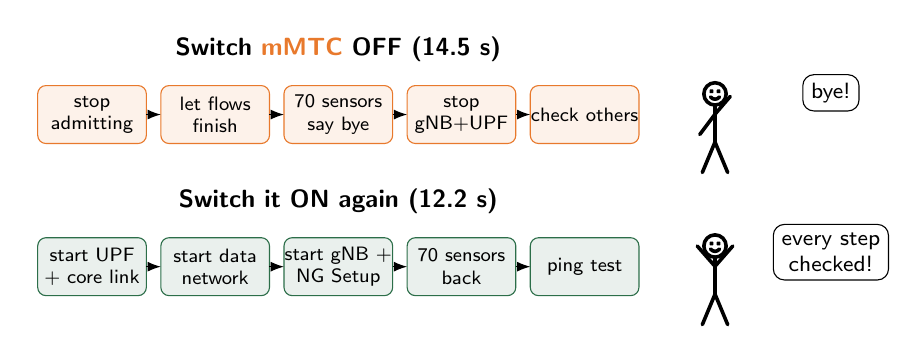
\begin{tikzpicture}[scale=0.92]
  \node[font=\bfseries\small] at (3.4,3.0) {Switch \textcolor{cM}{mMTC} OFF (14.5 s)};
  \foreach \t/\x in {stop admitting/0, let flows finish/1.7, 70 sensors say bye/3.4, stop gNB+UPF/5.1, check others/6.8}
    { \draw[cM,fill=cM!10,rounded corners=3pt] (\x-0.75,1.7) rectangle (\x+0.75,2.5);
      \node[font=\scriptsize,align=center,text width=1.4cm] at (\x,2.1) {\t}; }
  \foreach \x in {0.75,2.45,4.15,5.85} \draw[-{Latex}] (\x,2.1) -- (\x+0.2,2.1);
  \person[scale=0.7]{8.6,1.3}{w}
  \say{10.2,2.4}{bye!}
  \node[font=\bfseries\small] at (3.4,0.9) {Switch it ON again (12.2 s)};
  \foreach \t/\x in {start UPF + core link/0, start data network/1.7, start gNB + NG Setup/3.4, 70 sensors back/5.1, ping test/6.8}
    { \draw[ok,fill=ok!10,rounded corners=3pt] (\x-0.75,-0.4) rectangle (\x+0.75,0.4);
      \node[font=\scriptsize,align=center,text width=1.4cm] at (\x,0) {\t}; }
  \foreach \x in {0.75,2.45,4.15,5.85} \draw[-{Latex}] (\x,0) -- (\x+0.2,0);
  \person[scale=0.7]{8.6,-0.8}{u}
  \say{10.2,0.2}{every step\\checked!}
\end{tikzpicture}
\end{center}

\begin{tabularx}{\linewidth}{@{}Xcc@{}}
\toprule
& \textbf{mMTC on} & \textbf{mMTC off} \\ \midrule
mMTC sessions in the core & 70 & \textbf{0} \\
eMBB / URLLC devices still online & 20 / 10 & \textbf{20 / 10} \\
UE container CPU / memory & 211\,\% / 200 MiB & \textbf{\color{ok}40\,\% / 75 MiB} \\
a sensor asks for service & admitted & refused: ``mMTC is not active'' \\
\bottomrule
\end{tabularx}
\proof{docs/evidence/open5gs-network-orchestrator/1-lifecycle.txt}

While all this happened, URLLC's latency probes lost \textbf{0 of 63\,891} packets (p95 2.8 ms):
switching one slice did not disturb the others.

\shot{0.82}{14-slice-active-or-dormant.png}{Grafana, live run (section 9): each slice serving (1) or dormant (0). mMTC goes off at 16:07:56 and back on at 16:09:30; eMBB and URLLC stay at 1 (their lines overlap).}
\shot{0.82}{15-ues-and-core-sessions-per-slice.png}{Devices online per slice and the core's own session count. mMTC's devices go 70 → 0 → 70. In this run, under heavy load, the core still counted 11 mMTC sessions while the slice was off (see section 10).}

% ═════════════════════════ 6 rollback ═════════════════════════
\medskip
\section{Road builder: when something goes wrong, undo it}

\begin{center}
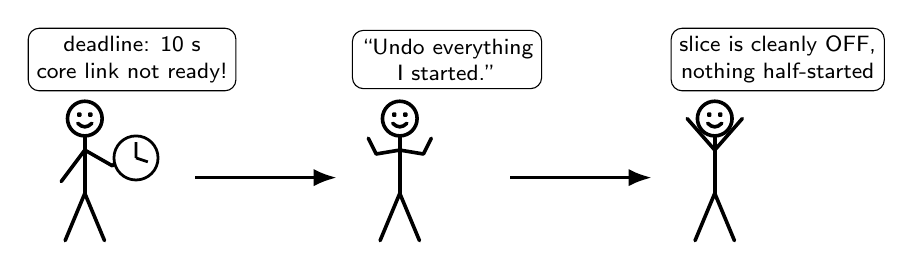
\begin{tikzpicture}
  \person{0,0}{h}
  \draw[line width=1pt,fill=white] (0.65,1.05) circle (0.28);
  \draw[line width=1pt] (0.65,1.05) -- (0.65,1.25) (0.65,1.05) -- (0.8,1.0);
  \say{0.6,2.3}{deadline: 10 s\\core link not ready!}
  \draw[-{Latex},line width=1.2pt] (1.4,0.8) -- (3.2,0.8);
  \person{4,0}{s}
  \say{4.6,2.3}{``Undo everything\\I started.''}
  \draw[-{Latex},line width=1.2pt] (5.4,0.8) -- (7.2,0.8);
  \person{8,0}{u}
  \say{8.8,2.3}{slice is cleanly OFF,\\nothing half-started}
\end{tikzpicture}
\end{center}

We gave an activation an impossible deadline (10 s). The core had not linked to the new UPF in
time, so the road builder \textbf{rolled back in 11.2 s}: it stopped the UPF it had just started.
mMTC was left cleanly off (0 containers running) and the other slices kept every device. A normal
activation right after worked in 12.1 s.

\proof{docs/evidence/open5gs-network-orchestrator/2-rollback.txt}

% ═════════════════════════ 7 closed loop ═════════════════════════
\section{Road builder: doing it on its own (closed loop)}

\begin{center}
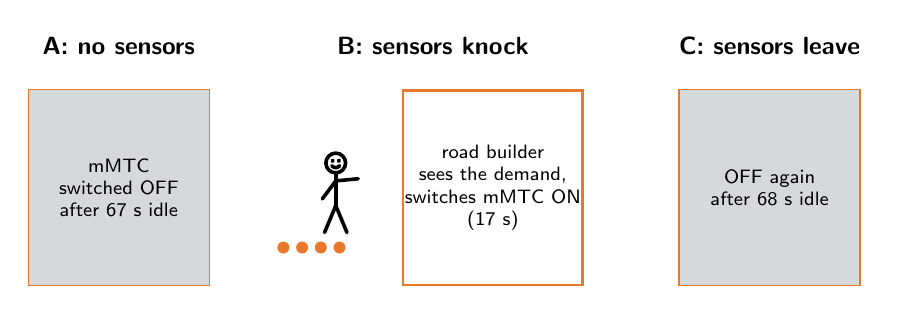
\begin{tikzpicture}[scale=0.95]
  % phase A
  \node[font=\bfseries\small] at (1.4,3.2) {A: no sensors};
  \draw[cM,line width=1pt] (0.2,0) rectangle (2.6,2.6); \fill[grey!25] (0.2,0) rectangle (2.6,2.6);
  \node[font=\scriptsize,align=center] at (1.4,1.3) {mMTC\\switched OFF\\after 67 s idle};
  % phase B
  \node[font=\bfseries\small] at (5.6,3.2) {B: sensors knock};
  \foreach \i in {0,...,3} \fill[cM] (3.6+\i*0.25,0.5) circle (0.08);
  \person[scale=0.6]{4.3,0.7}{p}
  \draw[cM,line width=1pt] (5.2,0) rectangle (7.6,2.6);
  \node[font=\scriptsize,align=center] at (6.4,1.3) {road builder\\sees the demand,\\switches mMTC ON\\(17 s)};
  % phase C
  \node[font=\bfseries\small] at (10.1,3.2) {C: sensors leave};
  \draw[cM,line width=1pt] (8.9,0) rectangle (11.3,2.6); \fill[grey!25] (8.9,0) rectangle (11.3,2.6);
  \node[font=\scriptsize,align=center] at (10.1,1.3) {OFF again\\after 68 s idle};
\end{tikzpicture}
\end{center}

With the closed loop on, the road builder reads the traffic cop's plan every few seconds.
mMTC (our ``on-demand'' slice) is switched on when sensors need it and off when they have been
quiet for a while. The sensors' requests in phase B, in order (\textcolor{bad}{r} refused,
\textcolor{ok}{A} admitted):

{\footnotesize\ttfamily\color{bad}rrrrrrrrrrrrrrrrrrrrr\color{ok}AAAAAAAAAAAAAAAAAAA\\AAAAAAAAAAAAAAAAAAAAAAAAAAAAAAAAAAAAAAAA\\AAAAAAAAAAAAAAAAAAAAAA}

21 were refused while the slice came up, then all 81 after that were admitted. The refused ones
are what woke it up: refused demand still counts in the plan.
\proof{docs/evidence/open5gs-network-orchestrator/3-closed-loop.txt}

% ═════════════════════════ 8 compute ═════════════════════════
\section{Road builder: how much CPU each slice gets}

\begin{center}
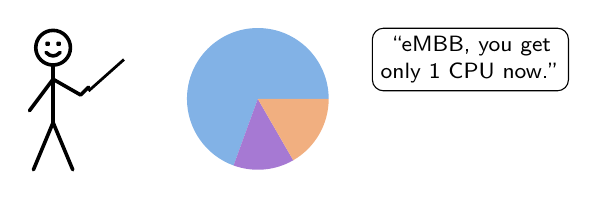
\begin{tikzpicture}
  \person{0,0}{h}
  \draw[line width=1pt] (0.45,1.0) -- (0.9,1.4);
  \fill[cE!60] (2.6,0.9) -- ++(0:0.9) arc (0:250:0.9) -- cycle;
  \fill[cU!60] (2.6,0.9) -- ++(250:0.9) arc (250:300:0.9) -- cycle;
  \fill[cM!60] (2.6,0.9) -- ++(300:0.9) arc (300:360:0.9) -- cycle;
  \say{5.3,1.4}{``eMBB, you get\\only 1 CPU now.''}
\end{tikzpicture}
\end{center}

\begin{tabularx}{\linewidth}{@{}Xcc@{}}
\toprule
\textbf{CPU for eMBB's gNB + UPF} & \textbf{eMBB carried} & \textbf{URLLC p99 meanwhile} \\ \midrule
unlimited & 366 Mbps & 11.0 ms \\
1 CPU & 121 Mbps & 10.4 ms \\
0.5 CPU & 50 Mbps & 8.1 ms \\
\bottomrule
\end{tabularx}
\proof{docs/evidence/open5gs-network-orchestrator/4-compute.txt}

The knob works: eMBB's capacity follows its CPU. URLLC improves only a little, so whether to use
it is a policy decision. By default eMBB is unlimited.

% ═════════════════════════ 9 live run ═════════════════════════
\newpage
\section{The photos: one live run, minute by minute}

All the Grafana screenshots in this document come from \textbf{one scripted 5-minute run} on
8 October (16:07--16:12 UTC), so they show the same events. The numbers in the tables above come
from the separate, longer evidence runs; this run is here so you can \emph{see} it happen.

\begin{center}
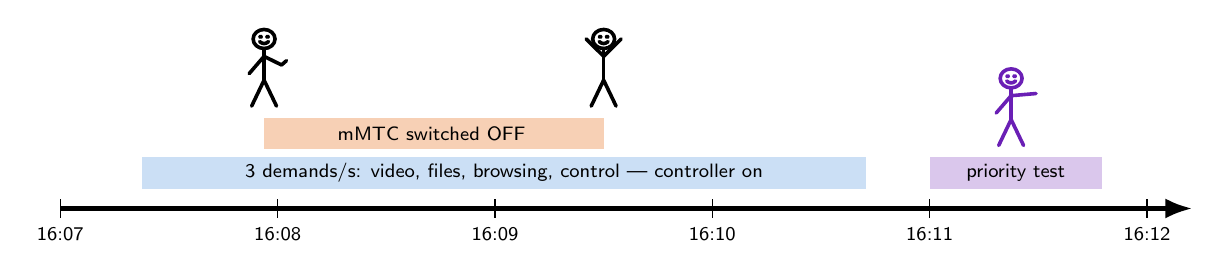
\begin{tikzpicture}[x=1.15cm]
  \draw[line width=1.5pt,-{Latex}] (0,0) -- (12.5,0);
  \foreach \x/\t in {0/16:07, 2.4/16:08, 4.8/16:09, 7.2/16:10, 9.6/16:11, 12/16:12}
    { \draw (\x,0.12) -- (\x,-0.12); \node[font=\scriptsize,below] at (\x,-0.12) {\t}; }
  \fill[cE!25] (0.9,0.25) rectangle (8.9,0.65); \node[font=\scriptsize] at (4.9,0.45) {3 demands/s: video, files, browsing, control — controller on};
  \fill[cM!35] (2.25,0.75) rectangle (6.0,1.15); \node[font=\scriptsize] at (4.1,0.95) {mMTC switched OFF};
  \fill[cU!25] (9.6,0.25) rectangle (11.5,0.65); \node[font=\scriptsize] at (10.55,0.45) {priority test};
  \person[scale=0.55]{2.25,1.3}{h} \person[scale=0.55]{6.0,1.3}{u} \person[scale=0.55,cU]{10.5,0.8}{p}
\end{tikzpicture}
\end{center}

\begin{tabularx}{\linewidth}{@{}lX@{}}
\toprule
\textbf{Time (UTC)} & \textbf{What happened} \\ \midrule
16:07:25 & demand starts; the controller soon cuts eMBB's limit (500 → 320 → 120 Mbps) as URLLC p95 jumps to 17.6 ms \\
16:07:56 & road builder switches mMTC off: done in 31.7 s (it waited for the busy host) \\
16:09:30 & mMTC on again: done in 16.0 s \\
16:10:45 & demand ends: 215 admitted, 265 refused (the controller and the dormant slice refused them) \\
16:11:20 & priority test: 20 standard URLLC demands, then 5 critical ones \\
\bottomrule
\end{tabularx}

\begin{center}
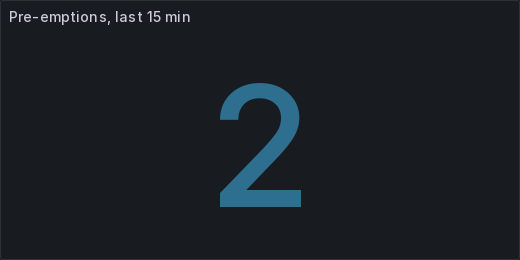
\includegraphics[width=0.32\linewidth]{16-stat-preemptions.png}\hfill
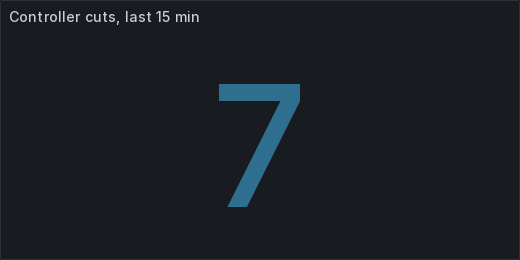
\includegraphics[width=0.32\linewidth]{17-stat-controller-cuts.png}\hfill
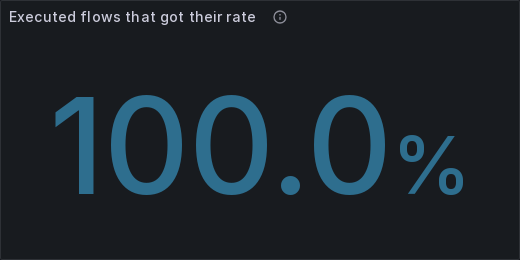
\includegraphics[width=0.32\linewidth]{20-flows-that-got-their-rate.png}\\[4pt]
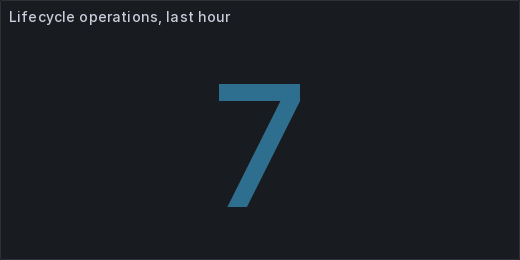
\includegraphics[width=0.32\linewidth]{18-stat-lifecycle-operations.png}\hfill
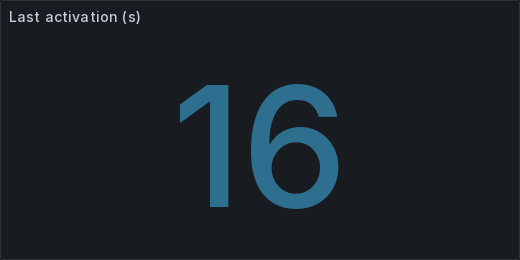
\includegraphics[width=0.32\linewidth]{19-stat-last-activation-seconds.png}\hfill
\hspace*{0.32\linewidth}
\end{center}
\begin{center}\footnotesize Counters from the same run: pre-emptions, controller cuts, executed flows that got their rate, lifecycle operations, and the last activation's time in seconds.\end{center}

\shot{0.82}{11-urllc-capacity-limit-admitted-measured.png}{URLLC in the same run: what was admitted and measured on the fast lane (capacity 20 Mbps).}

\shot{0.8}{21-prometheus-netorch-target-up.png}{Prometheus scraping both orchestrators: \texttt{network-orchestrator} (:9113) and \texttt{slice-orchestrator} (:9111) are UP.}

% ═════════════════════════ 10 what went wrong ═════════════════════════
\newpage
\section{Things that went wrong (and what we learned)}

\begin{center}
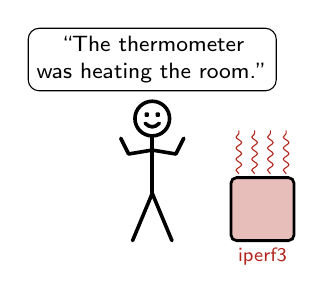
\begin{tikzpicture}
  \person{0,0}{s}
  \say{0,2.3}{``The thermometer\\was heating the room.''}
  \draw[line width=1pt,fill=bad!30,rounded corners=2pt] (1.0,0) rectangle (1.8,0.8);
  \foreach \x in {1.1,1.3,1.5,1.7} \draw[bad,decorate,decoration={snake,amplitude=1pt,segment length=4pt}] (\x,0.85) -- (\x,1.4);
  \node[font=\scriptsize,bad] at (1.4,-0.2) {iperf3};
\end{tikzpicture}
\end{center}

\begin{tabularx}{\linewidth}{@{}>{\raggedright\arraybackslash}p{4.3cm}X@{}}
\toprule
\textbf{Problem} & \textbf{What it did, and the fix} \\ \midrule
Our traffic tool was a CPU hog & iperf3's UDP sender used 45–90\,\% of a CPU core \emph{per flow}, at any speed. The load it put on the laptop is what made URLLC slow, so the first two versions of the controller looked broken and even blamed the wrong slice. Fix: our own light flow tool (1–10\,\% of a core). The bad runs are kept, clearly marked as superseded. \\
Leaked processes & A timed-out flow left its sender running for 5 minutes at 90\,\% CPU. Fix: every flow runs under a hard kill timer. \\
Port clash & Flows were given the same port as our KPI collector, so 7 of 26 failed instantly. Fix: flows use ports from 5410. \\
Lost commands to devices & The UE command tool sent ``deregister'' to stale entries of old processes, so 38 of 70 never arrived. Fix: stale entries are cleaned by checking which ports are really in use. \\
Sessions left in the core & Devices were killed before their ``I'm leaving'' message went out. Fix: let each device switch itself off first. Now the core frees 69–70 of 70. \\
``Unlimited CPU'' did nothing & \texttt{docker update --cpus 0} is silently ignored, but we reported success. Fix: unlimited = all 12 cores, and every change is read back. \\
Kubernetes would have broken & The UE pod would not have found its new helper script. Fixed in the generated manifests, not yet run on minikube. \\
Stale sessions under heavy load & In the live run (section 9), with the host busy, 11 of 70 sensors stopped before their ``leaving'' message reached the core, so the core kept counting them while mMTC was off. They clear when the sensors come back. Not fixed: switching off now reports it as a clear \textbf{WARNING} instead of a quiet detail. \\
\bottomrule
\end{tabularx}

\begin{keybox}
\textbf{The lesson for all of us:} before trusting a measurement, check what the measuring tool
itself costs. Every run now records the host's load and any leftover processes.
\end{keybox}

% ═════════════════════════ 10 proofs ═════════════════════════
\section{Where every proof lives}

\begin{tabularx}{\linewidth}{@{}>{\raggedright\arraybackslash\footnotesize\ttfamily}p{7.2cm}X@{}}
\toprule
\normalfont\normalsize\textbf{Folder / file} & \textbf{What is inside} \\ \midrule
docs/evidence/\newline open5gs-orchestrator-dynamic/ & priority, controller on/off, planning, diagnosis — every flow and every controller decision as JSON \\
docs/evidence/\newline open5gs-network-orchestrator/ & off/on, rollback, closed loop, compute — every operation with its step timings \\
docs/evidence/open5gs-orchestrator-dynamic/\newline superseded-iperf3-load/ & the runs spoiled by iperf3 — kept on purpose, do \textbf{not} quote them \\
docs/screenshots/open5gs/10-*.png to 21-*.png & the Grafana screenshots in this document \\
docs/adr/ADR-016-dynamic-slice-allocation.md & the traffic cop's design decisions \\
docs/adr/ADR-017-network-orchestrator.md & the road builder's design decisions \\
\bottomrule
\end{tabularx}

\textbf{To see it yourself} (on the lab machine, stack running):

{\footnotesize
\begin{tabularx}{\linewidth}{@{}>{\ttfamily}p{9.4cm}X@{}}
make o5gs-network & state of every slice \\
python3 tools/network-orchestrator/netorch.py deactivate mMTC & switch a slice off \\
python3 tools/network-orchestrator/netorch.py activate mMTC & \ldots and on again \\
make o5gs-dynamic & re-run the traffic cop experiments ($\approx$25 min) \\
make o5gs-network-demo & re-run the road builder experiments ($\approx$16 min) \\
http://localhost:3001 (Grafana) & rows ``Dynamic allocation'' and ``Network orchestrator'' \\
\end{tabularx}}

\textbf{Still provisional — to confirm with our guide:} 3 critical / 7 standard URLLC devices;
the controller's 8 ms / 5 ms lines; mMTC as the only on-demand slice; 120 s idle time; 150 s
activation deadline.

\vspace{6pt}
\begin{center}
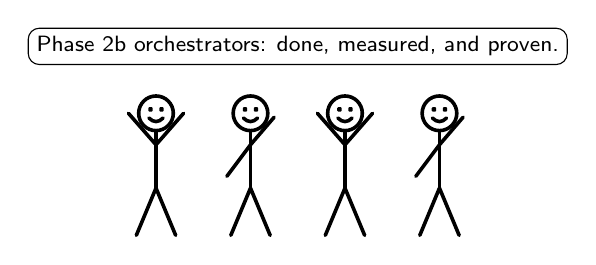
\begin{tikzpicture}
  \person{0,0}{u} \person{1.2,0}{w} \person{2.4,0}{u} \person{3.6,0}{w}
  \say{1.8,2.4}{Phase 2b orchestrators: done, measured, and proven.}
\end{tikzpicture}
\end{center}

\end{document}
